\section{\ExercisePrefixMemory Zeiger und Referenzen Grundlagen}
\label{sec:pointers}
\cpppSolutionName{pointers}{pointers}
In dieser Aufgabe sollst du den Umgang mit Zeigern (\emph{Pointer}) und Referenzen erlernen.
Diese erlauben es zum Beispiel Werte zwischen Funktionen auszutauschen, ohne eine Kopie der zu übermittelnden Daten zu erzeugen.
Anstelle dessen kann ein (vergleichsweise kleiner) Zeiger auf einen Speicherbereich übergeben werden.
Alternativ kann auch eine Referenz auf eine Variable übergeben werden, welche intern ähnlich wie ein Zeiger gehandhabt wird.

\subsection{Experimente}
Experimentiere mit Zeigern, Adressen und Referenzen. Als Ausgangsbasis kann folgendes Programmfragment dienen.
Fülle danach die untenstehende Skizze aus, um dir klarzumachen, wie Variablen und ihre Speicherabbilder zusammenhängen.

\cpppInputListing{02_memory/problems/listings/pointers_intro.cpp}

\paragraph{Speicherabbild}
Wir nehmen an, dass Speicheradressen immer 4 Byte (= 32 Bit) breit sind. 
Trage nun die auftretenden Variablen \lstinline{intVal} und \lstinline{pIntVal} mit den folgenden Eigenschafen in das Speicherabbild ein.
\begin{itemize}
	\item Typ, Name und Wert jeder Variablen
	\item Speicheradressen in Bytes (Die Speicheradressen kannst du frei wählen, der Pointer sollte aber natürlich auf die entsprechend gewählte Adresse zeigen.)
	\item Der Wert, der an der jeweiligen Speicheradresse steht.
\end{itemize}

\begin{center}
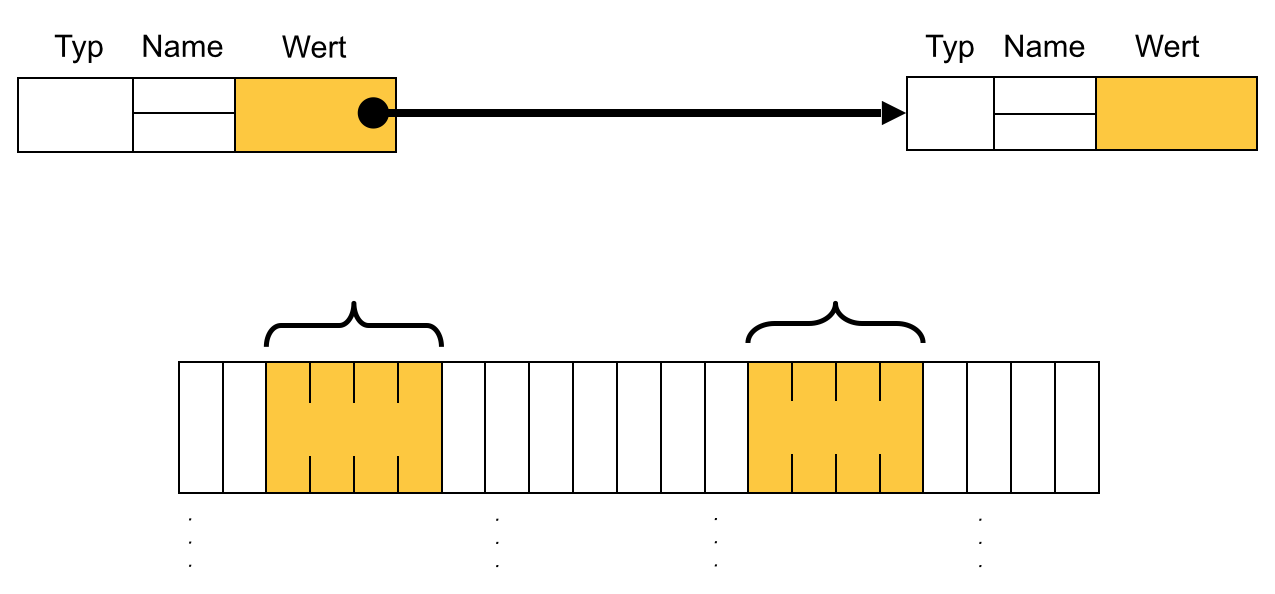
\includegraphics[width=.9\textwidth]{02_memory/figures/memory_image.png}
\end{center}

\subsection{Bedeutung von Variablentypen verstehen}
Versuche die Bedeutung folgender Ausdrücke zu verstehen.
Welche Regelmäßigkeiten stellst du fest?

\cpppInputNoPageBreakListing{02_memory/problems/listings/pointers_intro_advanced.cpp}

\hints{
	\item Gehe beim Interpretieren von Variablentypen von Rechts nach Links vor.
}

\subsection{Gültigkeit}
Warum sind folgende Ausdrücke ungültig, sinnlos oder sogar gefährlich?

\cpppInputListing{02_memory/problems/listings/pointers_intro_validity.cpp}

\hints{
	\item Finde heraus, welchen Typ der Ausdruck hätte haben müssen.
	\item Nur tatsächlich angelegte Variablen haben Adressen. Ausdrücke wie a + b oder direkt kodierte Zahlenliterale wie 42 haben keine Adresse.
}

\subsection{Variablentausch}
Schreibe eine Funktion \lstinline{swap}, die zwei \lstinline{int}-Variablen miteinander vertauscht.
Probiere dabei beide möglichen Übergabevarianten (per Referenz, per Pointer) aus.
Was würde passieren, wenn man die Variablen stattdessen per Wert übergeben würde?

\subsection{Programmanalyse}
Sieh dir folgendes Programm an.

\cpppInputNoPageBreakListing{02_memory/problems/listings/pointers_programm.cpp}

Welche Ausgaben werden übereinstimmen, welche werden sich unterscheiden?
Führe das Programm aus.
Hast du diese Ausgabe erwartet?

\subsection{Const Correctness}

In dieser Aufgabe setzt du dich mit der Bedeutung des Schlüsselworts \lstinline{const} im Kontext von Pointern auseinander.

Versuche für jede der Variablen im folgenden Code je eine \emph{Verwendung} zu finden, die  
\begin{itemize}
\item gültig ist (= fehlerfrei kompiliert) und
\item nicht gültig ist (= einen Compiler-Fehler wirft).
\end{itemize}


Was ist jeweils der Grund?
Welche Pointer verhalten sich gleich?

\cpppInputNoPageBreakListing{02_memory/problems/listings/pointers_behavior.cpp}

\paragraph{Mehrstufige Pointer}

Versuche nun das Gleiche mit den folgenden mehrstufigen Pointern.

\cpppInputNoPageBreakListing{02_memory/problems/listings/pointers_multi.cpp}

\subsection{Übergabewerte}
In dieser Aufgabe geht es darum, das gerade erlangte Verständnis über Pointer und Referenzen zu festigen und zu kontrollieren.
In Tabelle \ref{table:uebergabewerte} sind in der ersten Spalte Funktionen mit verschiedenen Parametern gegeben.
In der ersten Zeile findest du verschiedene Variablentypen.
Deine Aufgabe ist es nun, zu den verschiedenen Funktionen die passenden Parameter aus den Variablen herzustellen.
Falls eine Variable nicht verwendet werden kann, trage bitte ein \xmark ein. \\\\
Als Beispiel dient die erste Zeile. 

\begin{table}[h]
    \centering

    \newcolumntype{b}{X}
    \newcolumntype{s}{>{\hsize=.6\hsize}X}

    \begin{tabularx}{\textwidth}{b *5{| >{\centering\arraybackslash}s}@{}} 
       & \lstinline!int i! & \lstinline!int *j! & \lstinline!int const * const k!  & \lstinline!int **l! & \lstinline!const int *m! \\
	    \hline
		\mbox{\lstinline!op1(int *)!}          & \mbox{\lstinline!&i!} & \mbox{\lstinline!j!} & \xmark & \mbox{\lstinline!*l!} & \xmark \\ 
		\hline
		\mbox{\lstinline!op2(int)!}            & & & & & \\ 
		\hline
		\mbox{\lstinline!op3(int &)!}         & & & & & \\ 
		\hline
		\mbox{\lstinline!op4(const int **)!}   & & & & & 
    \end{tabularx}
    \caption{Tabelle für \emph{Übergabewerte} Aufgabe}
    \label{table:uebergabewerte}
\end{table}
